\documentclass{article}
\usepackage{tikz}
\usetikzlibrary{arrows.meta}

\begin{document}

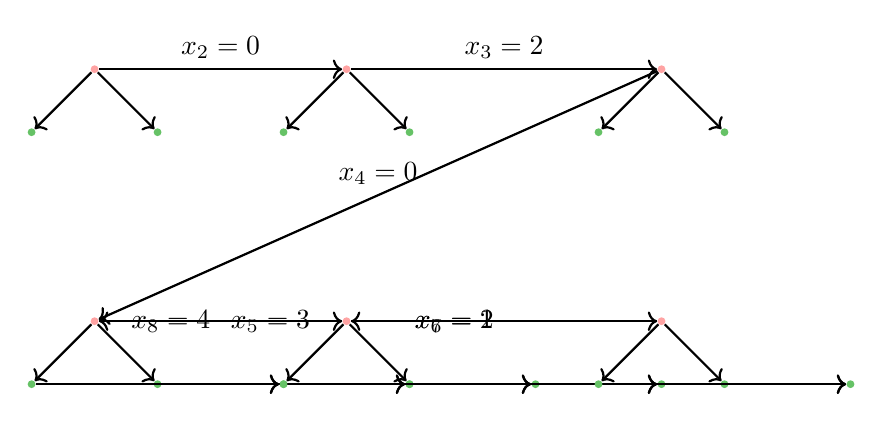
\begin{tikzpicture}[scale=0.8]
    % Define colors
    \definecolor{red}{RGB}{255, 102, 102}
    \definecolor{green}{RGB}{0, 153, 0}
    
    % Nodes for the first tree
    \node[circle, fill=red!60, inner sep=1pt] (root1) at (0,0) {};
    \node[circle, fill=green!60, inner sep=1pt] (child1) at (-1,-1) {};
    \node[circle, fill=green!60, inner sep=1pt] (child2) at (1,-1) {};
    
    % Draw edges for the first tree
    \draw[->, thick] (root1) -- (child1);
    \draw[->, thick] (root1) -- (child2);
    
    % Nodes for the second tree
    \node[circle, fill=red!60, inner sep=1pt] (root2) at (4,0) {};
    \node[circle, fill=green!60, inner sep=1pt] (child3) at (3,-1) {};
    \node[circle, fill=green!60, inner sep=1pt] (child4) at (5,-1) {};
    
    % Draw edges for the second tree
    \draw[->, thick] (root2) -- (child3);
    \draw[->, thick] (root2) -- (child4);
    
    % Nodes for the third tree
    \node[circle, fill=red!60, inner sep=1pt] (root3) at (9,0) {};
    \node[circle, fill=green!60, inner sep=1pt] (child5) at (8,-1) {};
    \node[circle, fill=green!60, inner sep=1pt] (child6) at (10,-1) {};
    
    % Draw edges for the third tree
    \draw[->, thick] (root3) -- (child5);
    \draw[->, thick] (root3) -- (child6);
    
    % Nodes for the fourth tree
    \node[circle, fill=red!60, inner sep=1pt] (root4) at (0,-4) {};
    \node[circle, fill=green!60, inner sep=1pt] (child7) at (-1,-5) {};
    \node[circle, fill=green!60, inner sep=1pt] (child8) at (1,-5) {};
    \node[circle, fill=green!60, inner sep=1pt] (child9) at (3,-5) {};
    \node[circle, fill=green!60, inner sep=1pt] (child10) at (5,-5) {};
    
    % Draw edges for the fourth tree
    \draw[->, thick] (root4) -- (child7);
    \draw[->, thick] (root4) -- (child8);
    \draw[->, thick] (child7) -- (child9);
    \draw[->, thick] (child7) -- (child10);
    \draw[->, thick] (child8) -- (child9);
    \draw[->, thick] (child8) -- (child10);
    
    % Nodes for the fifth tree
    \node[circle, fill=red!60, inner sep=1pt] (root5) at (4,-4) {};
    \node[circle, fill=green!60, inner sep=1pt] (child11) at (3,-5) {};
    \node[circle, fill=green!60, inner sep=1pt] (child12) at (5,-5) {};
    \node[circle, fill=green!60, inner sep=1pt] (child13) at (7,-5) {};
    \node[circle, fill=green!60, inner sep=1pt] (child14) at (9,-5) {};
    
    % Draw edges for the fifth tree
    \draw[->, thick] (root5) -- (child11);
    \draw[->, thick] (root5) -- (child12);
    \draw[->, thick] (child11) -- (child13);
    \draw[->, thick] (child11) -- (child14);
    \draw[->, thick] (child12) -- (child13);
    \draw[->, thick] (child12) -- (child14);
    
    % Nodes for the sixth tree
    \node[circle, fill=red!60, inner sep=1pt] (root6) at (9,-4) {};
    \node[circle, fill=green!60, inner sep=1pt] (child15) at (8,-5) {};
    \node[circle, fill=green!60, inner sep=1pt] (child16) at (10,-5) {};
    \node[circle, fill=green!60, inner sep=1pt] (child17) at (12,-5) {};
    
    % Draw edges for the sixth tree
    \draw[->, thick] (root6) -- (child15);
    \draw[->, thick] (root6) -- (child16);
    \draw[->, thick] (child15) -- (child17);
    \draw[->, thick] (child16) -- (child17);
    
    % Arrows and labels
    \draw[->, thick] (root1) -- node[above] {$x_2 = 0$} (root2);
    \draw[->, thick] (root2) -- node[above] {$x_3 = 2$} (root3);
    \draw[->, thick] (root3) -- node[above] {$x_4 = 0$} (root4);
    \draw[->, thick] (root4) -- node[right] {$x_5 = 3$} (root5);
    \draw[->, thick] (root5) -- node[left] {$x_6 = 1$} (root6);
    \draw[->, thick] (root6) -- node[left] {$x_7 = 2$} (root5);
    \draw[->, thick] (root5) -- node[left] {$x_8 = 4$} (root4);
\end{tikzpicture}

\end{document}